% !TeX root = ../Book2.tex
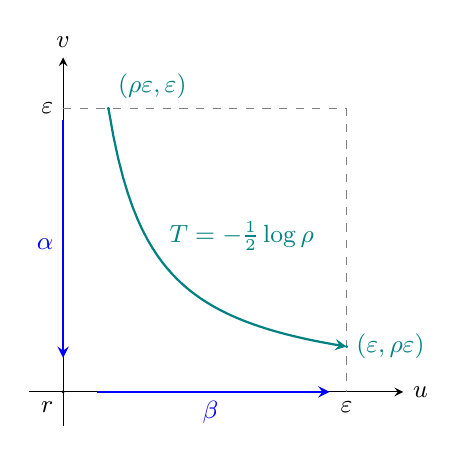
\begin{tikzpicture}[x=3.6cm,y=3.6cm,>=stealth,font=\small]
	\draw[->] (-0.12,0) -- (1.2,0) node[right] {\(\lVert u\rVert\)};
	\draw[->] (0,-0.12) -- (0,1.18) node[above] {\(\lVert v\rVert\)};
	\draw[dashed,gray] (0,1) -- (1,1) -- (1,0);
	\draw[thick,blue,->] (0,0.96) -- (0,0.12);
	\draw[thick,blue,->] (0.12,0) -- (0.94,0);
	\draw[thick,teal,->,domain=0.16:1,samples=50] plot (\x,{0.16/\x});
	\fill[teal] (0.16,1) circle (0.6pt) node[above right] {\((\rho\varepsilon,\varepsilon)\)};
	\fill[teal] (1,0.16) circle (0.6pt) node[right] {\((\varepsilon,\rho\varepsilon)\)};
	\fill (0,0) circle (0.6pt) node[below left] {\(r\)};
	\node[left] at (0,1) {\(\varepsilon\)};
	\node[below] at (1,0) {\(\varepsilon\)};
	\node[left,blue] at (0,0.52) {\(\alpha\)};
	\node[below,blue] at (0.52,0) {\(\beta\)};
	\node[teal] at (0.63,0.55) {\(T=-\frac12\log\rho\)};
\end{tikzpicture}
